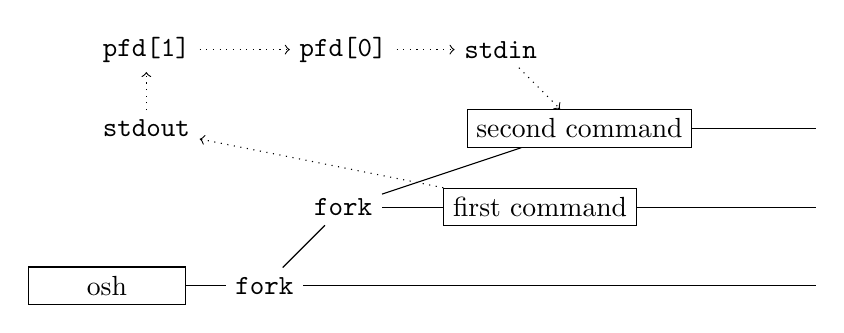
\begin{tikzpicture}
\tikzstyle{process} = [minimum width=2cm,draw,];
\tikzstyle{thread} = [minimum width=2cm,draw,dashed]
\tikzstyle{message} = [->,dotted];

\node [process] (v1) at (-3.5,0) {osh};
\node [process] (v2) at (2,1) {first command};
\node [process] (v5) at (2.5,2) {second command};

\node (v3) at (-1.5,0) {\texttt{fork}};
\draw  (v1) edge (v3);
%\draw  (v3) edge (v2);
\node (v4) at (-0.5,1) {\texttt{fork}};
%\draw  (v2) edge (v4);
\draw  (v4) edge (v5);
\draw (v3) -> (5.5,0);
%\draw (v4) -> (3,1);
\draw (v5) -> (5.5,2);
\node (v7) at (-3,3) {\texttt{pfd[1]}};
\node (v6) at (-3,2) {\texttt{stdout}};
\node (v8) at (-0.5,3) {\texttt{pfd[0]}};
\node (v9) at (1.5,3) {\texttt{stdin}};
\draw [message] (v2) edge (v6);
\draw [message] (v6) edge (v7);
\draw [message] (v7) edge (v8);
\draw [message] (v8) edge (v9);
\draw [message] (v9) edge (v5);
\draw  (v3) edge (v4);
\draw  (v4) edge (v2);
\draw (v2) -- (5.5,1);
\end{tikzpicture}